\section{Introduction}\label{sec:intro}


In an era marked by the rapid evolution of Artificial General Intelligence (AGI), there emerged many fantastic applications with AGI techniques such as ChatGPT in Natural Language Processing (NLP) and Midjourney in Computer Vision (CV). AGI has greatly improved our lives, making our work more efficient and freeing us from repetitive tasks to focus on more creative endeavors. However, when it comes to working with graph data, AGI applications are still in their early stages compared with the huge success in NLP \cite{
devlin2019bert, 
brown2020language, liu2023pretrain} and CV areas \cite{
% radford2021learning, 
% li2022blip, 
% zhu2023minigpt4, 
wang2023chatvideo, 
zhang2023videollama}. In our increasingly interconnected world, understanding and extracting valuable insights from graphs is crucial. This places AGI applied to graph data at the forefront of both academic and industrial interest \cite{liu2023graph, zhang2023large, yang2023datacentric}, with the potential to redefine fields like drug design \cite{rong2020selfsupervised, qian2023can} and battery development \cite{wang2023scientific}, etc.




\begin{figure}[!t]
    \centering
    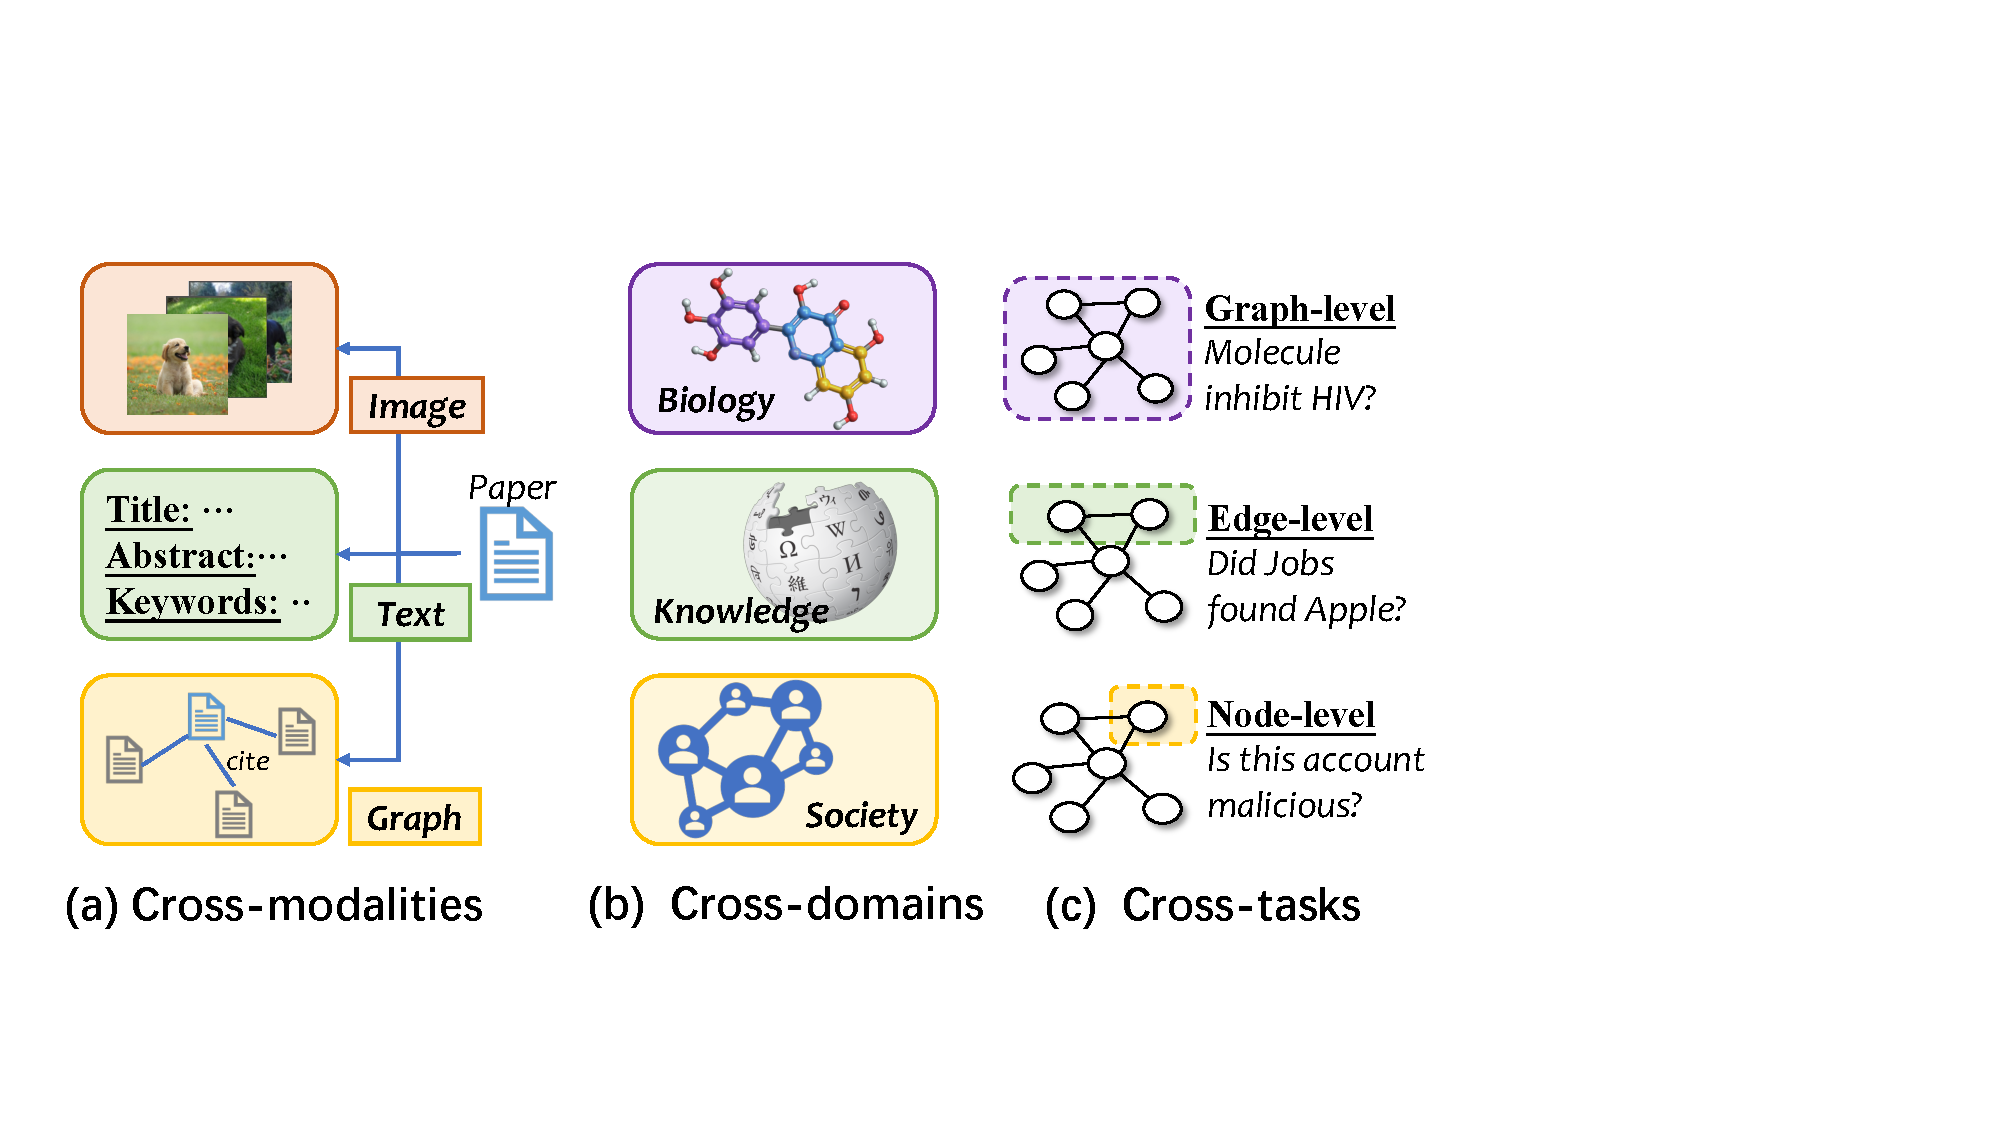
\includegraphics[width=0.45\textwidth]{pic/ThreeChallenges} 
    \caption{The Most Frequently Problems towards Artificial General Intelligence. (a) Cross-modalities, (b) Cross-domains, (c) Cross-tasks.}
    \label{fig:AGIProblems}
\end{figure}



However, realizing this vision is never easy. Figure \ref{fig:AGIProblems} illustrates this landscape for recent research in Artificial General Intelligence, from which we can see that there are at least three fundamental problems in technique: How to make the model general for different modalities, different domains, and different tasks? Within the NLP and CV areas, there have been many commercial models that can understand and translate information across these modalities \cite{
devlin2019bert, 
% radford2021learning, 
% li2022blip, 
% zhu2023minigpt4, 
zhang2023videollama, 
brown2020language}. For example, models like BERT \cite{devlin2019bert} and GPT-3 \cite{brown2020language} have demonstrated the ability to perform tasks that involve both textual and visual information. However, in the context of graph data, the harmonization of information from multiple modalities remains largely uncharted territory \cite{li2023graphadapter}.
% he2023explanations, 
% yoon2023multimodal, 
% li2023graphadapter
% chen2023exploring
For the cross-domain issue, transfer learning has proven effective, enabling models to apply knowledge learned from images and text in one domain to another. However, transferring knowledge between different graph domains is very tough because the semantic spaces are not aligned \cite{zhu2023graphcontrol} and the structural patterns are also not similar \cite{ zhao2023graphglow}, making graph domain adaptation remains a very frontier and not well-solved AGI problem. Currently, most graph research on transfer learning focuses on the third problem, how to leverage the pre-trained graph knowledge in the same graph domain to perform different graph tasks (like node classification, link prediction, graph classification, etc) \cite{sun2022gppt, liu2023graphprompt, sun2023all, fang2023universal, zhu2023sglpt, hu2020gptgnn, shirkavand2023deep, ge2023enhancing}. However, compared with the huge success in NLP and CV, task transferring within the same graph domain is still primitive with far fewer instances of successful industrial applications. While the AGI research boasts notable achievements in many linear data like images, 
% \cite{
% % radford2021learning, 
% li2022blip}, 
text \cite{robinson2023leveraging, devlin2019bert, brown2020language}, and videos \cite{wang2023chatvideo, zhang2023videollama}, the fundamental problems within the realm of graph data remain underexplored. Besides the above three foundation problems, Artificial General Intelligence has also encountered many social disputes. For example, training large foundation models consumes exorbitant amounts of energy and may yield unintended counterfactual outcomes \cite{liu2022ptuning, schick2021it}. These concerns have led to a growing consensus within the AI community on the efficient extraction of useful knowledge preserved by these large models, minimizing the need for repetitive fine-tuning across various downstream tasks \cite{gao2021making, lester2021power}. This consensus not only promises to alleviate the environmental impact but also offers a practical solution to the challenge of model efficiency and adaptability in an era of AGI.




At the core of recent AGI technology, prompt learning has presented huge potential to solve the above problems and demonstrated remarkable success in NLP and CV applications \cite{qin2021learning, tsimpoukelli2021multimodal, liu2023pretrain}. Prompt learning is the art of designing informative prompts  to manipulate input data for the pre-trained foundation models. Figure \ref{fig:PromptExample} shows an example of a textual-format prompt applied to a pre-trained language model to directly perform downstream inference tasks. By reformulating downstream tasks into pre-training tasks, this approach avoids the need for extensive model tuning and efficiently extracts preserved knowledge \cite{brown2020language, jiang2020how}. Since its powerful capabilities in data manipulation, task reformulation, and extraction of significant insights, prompting is very promising to address the aforementioned cross-modalities, cross-domains, and cross-task challenges in one way. Compared with large models, the prompt is usually very lightweight and can efficiently extract useful knowledge by reducing the extensive computational resources caused by repeat tuning of these large models \cite{lester2021power, shin2020autoprompt}. Intuitively, text and images can be perceived as specific instances of a more general graph data structure. For instance, a sentence can be treated as a graph path, with words as nodes, and an image can be viewed as a grid graph, where each pixel serves as a graph node. This insight encourages us to explore the transference of successful prompting techniques from text to the graph area for similar concerns. 


\begin{figure}[!t]
    \centering
    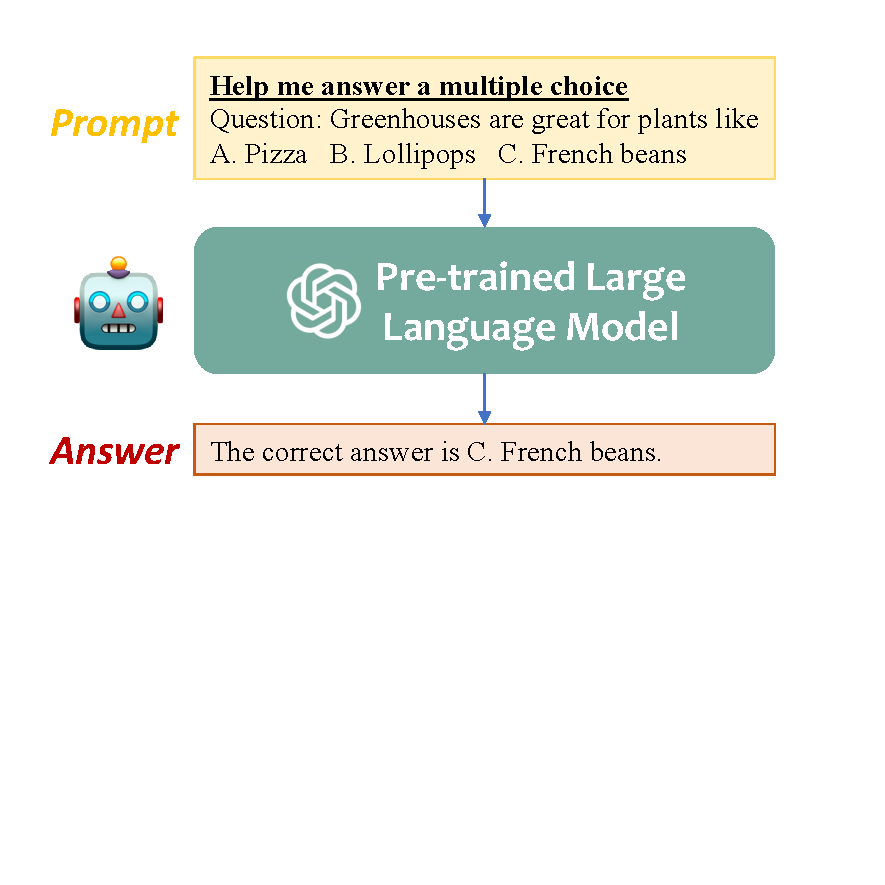
\includegraphics[width=0.45\textwidth]{pic/PromptExample.pdf} 
    \caption{An example of the language prompt. A textual prompt is designed to let the pre-trained large language model perform the multi-choice question-answering task.}
    \label{fig:PromptExample}
\end{figure}




Recently, some researchers have started to introduce prompt learning to graph data \cite{sun2022gppt, liu2023graphprompt, sun2023all, fang2023universal, zhu2023sglpt, ma2023hetgpt, guo2023datacentric, chen2023ultradp, gong2023prompt}. However, some further studies have found that the graph prompt is very different from their counterparts in the NLP area \cite{sun2023all}. First, the design of graph prompts proves to be a far more intricate endeavor compared to the formulation of language prompts. Classic language prompts often comprise predefined phrases or learnable vectors appended to input text \cite{brown2020language, gao2021making}. Here, the primary focus lies in the content of the language prompt. However, we actually do not know what a graph prompt looks like. A graph prompt not only contains the prompt "content" but also includes the undefined task of determining how to structure these prompt tokens and seamlessly integrate them into the original graph. Second, the harmonization of downstream graph problems with the pre-training task is more difficult than language tasks \cite{liu2023graphprompt, sun2023all}. For example, a typical pre-training approach for a language model is to predict a masked word by the model \cite{devlin2019bert}. Then many downstream tasks such as question answering, and sentiment classification can be easily reformulated as word-level tasks \cite{liu2023pretrain}. Unlike NLP, where pre-training tasks often share a substantial task sub-space, graph tasks span node-level \cite{grover2016node2vec}, edge-level \cite{zhang2018link}, and graph-level objectives \cite{sun2020infograph, sun2021heterogeneous}, making pre-training pretexts less adaptable. Third, compared with prompts in NLP which are usually some understandable phrases, graph prompts are usually less intuitive to non-specialists. The fundamental nature and role that graph prompts play within the graph model remain somewhat elusive without comprehensive theoretical analysis. There is also a lack of clear-cut evaluation criteria for the quality of designed graph prompts. In addition, there are still many unclear questions for us to further understand graph prompting. For example, how effective are these graph prompts? What is their efficiency in terms of parameter complexity and training burden? How powerful and flexible do these prompts manipulate the original graph data? In light of these intricacies questions, there is a pressing need for delving deeper into the potential of graph prompts in AGI, thereby paving the way for a more profound understanding of this evolving frontier within the broader data science landscape.




While there have been recent endeavors to explore graph prompting, a consistent framework or clear route remains unavailable. These efforts vary significantly in terms of perspective, methodology, and target tasks, which present a fragmented landscape of graph prompting and pose a considerable obstacle to the systematical advancement of this research area. There arises an urgent need to provide a panoramic view, analysis, and synthesis of the latest advances in this realm with a unified framework. In light of this situation, we offer this survey to present how existing work on graph prompts tries to solve the three foundation problems towards AGI as previously mentioned.  Beyond that, we also wish to push forward the research area by answering the following detailed research questions (RQs): 

\begin{itemize}
    \item \textbf{RQ1: How to understand existing work with a unified framework since they are very different?} Our main focus is to understand the various methods used in the field of graph prompting. We want to bring together all these different approaches and ideas to create a single, cohesive framework. This framework will help us thoroughly grasp the existing research and provide a strong foundation for future research in this area.
   \item  \textbf{RQ2: Why Prompt? What's the Nature of Graph Prompt?}
  In this part of our study, we aim to understand why prompts are important. We want to uncover the fundamental aspects of graph prompts. What exactly do graph prompts do in graph problems? How do they fit into the complex graphs, and how do they help us achieve the broader goal of creating AI systems that can handle graph data effectively? These questions highlight the significant role that graph prompts play in shaping the future of AI when dealing with graph information.

   
   \item  \textbf{RQ3: How to Design Graph Prompts?} Designing good graph prompts is a complex task. In this part, we explore the technical details of designing graph prompts: what do they look like, how do they align downstream tasks and the pre-train task, and how they are learned? These important questions focus on the skill of making prompts that work well with the complexities of graph data, helping researchers make better prompts.
   
   % \item  \textbf{RQ4: How to Evaluate the Quality of Graph Prompts?}
   % When it comes to graph prompts, it's not as straightforward as evaluating text prompts, which are more accessible to people who aren't experts. You can't easily judge the quality of a graph prompt just by looking at it. In this part of our research, we want to figure out how to measure how well graph prompts work, how efficiently they perform, how much power they have, how flexible they are, and whether they can be used in different situations. These questions are crucial for truly understanding the impact, potential, and limitations of prompts in the context of graph data.


   
   \item  \textbf{RQ4: How to Deploy Graph Prompts in Real-world Applications?} At the moment, there isn't an easy-to-use toolkit for creating graph prompts. The potential applications that graph prompts can be deployed are under-exploration. This research question focuses on making graph prompts practical for use in real-world situations with an easily extensible programming package. 

   
   \item  \textbf{RQ5: What Are the Current Challenges and Future Directions in Graph Prompting?} This question guides us to look at the challenges we're dealing with today and the way forward. By tackling these important questions, we hope to provide a roadmap for ongoing graph-prompting research. 

   
\end{itemize}




To answer the first research question (RQ1), we propose a unified framework to analyze graph prompt learning work. Our framework casts the concept of a graph prompt into prompt tokens, token structures, and inserting patterns. This higher-level perspective offers clarity and comprehensiveness, providing readers with a structured understanding of this burgeoning field. To the best of our knowledge, our survey marks the first of its kind to bring together these multifaceted aspects of graph prompting within a single unified framework.


To answer the second research question (RQ2), we explore the correlations between prompts and existing graph models through the lenses of flexibility and expressiveness and then present a fresh and insightful perspective to uncover the nature of graph prompts. Unlike most prompt learning surveys in NLP areas \cite{liu2023pretrain} that treat prompting as a trick of filling the gap between the pre-training tasks and downstream tasks, we reveal that graph prompts and graph models are interconnected on a deeper level. This novel perspective offers invaluable insights into why prompt learning holds promise in the graph area and what distinguishes it from traditional fine-tuning methods \cite{hu2020strategies}. To our knowledge, this is the first endeavor to offer such an illuminating perspective on graph prompting.


To answer the third research question (RQ3), we introduce a comprehensive taxonomy that includes more than 100 related works. Our taxonomy dissects these works, categorizing them according to node-level, edge-level, and graph-level tasks, thereby aligning them with the broader context of the pre-training task. This will empower our readers with a clearer comprehension of the mechanisms underlying prompts within the whole "pre-training and prompting" workflow.


%To answer the fourth research question (RQ4), we employ both quantitative and qualitative analyses to represent work on graph prompts. We designed a series of experiments aimed at comparing the efficiency and flexibility of these approaches. Notably, we introduce a novel metric, the "augmentation simulation error bound," designed to quantitatively assess a graph prompt's capacity for simulating various graph operations, such as node and edge dropping.


To answer the fourth research question (RQ4), we developed ProG (prompt graph) \footnote{\url{https://github.com/sheldonresearch/ProG}}, a unified Python library to support graph prompting. Additionally, we established a website\footnote{\url{https://github.com/WxxShirley/Awesome-Graph-Prompt}} that serves as a repository for the latest graph prompt research. This platform curates a comprehensive collection of research papers, benchmark datasets, and readily accessible code implementations. By providing this accessible ecosystem, we aim to empower researchers and practitioners to advance this burgeoning field more effectively. 

Beyond these, our survey goes a step further with an introduction of potential applications, a thoughtful analysis of the current challenges, and a discussion of future directions, thus providing a comprehensive roadmap for the evolution of this vibrant and evolving field (RQ5). Our contributions are summarised as follows:

\begin{itemize}
    \item \textbf{Enabling Comprehensive Analysis.} We propose a unified framework for analyzing graph prompt learning work, providing a comprehensive view of prompt tokens, token structures, and inserting patterns.     
    \item \textbf{Novel Perspectives on Prompt-Model Interplay. } We offer fresh insights into the nature of graph prompts. Unlike traditional work that simply treats prompts as a trick of filling the gap between downstream tasks and the pre-train task, we explore the flexibility and expressiveness issues of graph models and pioneer a more thorough perspective into the interplay between prompts and existing graph models.
    \item \textbf{A Systematic Taxonomy of Graph Prompting. }We systematically explore over a hundred recent works in the domain of graph prompting. This taxonomy not only organizes these contributions but also furnishes readers with a comprehensive understanding of prompt mechanisms within the overarching "pre-training and prompting" workflow.
    % \item \textbf{Quantitative and Qualitative Insights. } We conduct extensive experiments to evaluate different graph prompts and propose a new metric to evaluate how well a graph prompt reformulates graph data.
    \item \textbf{Empowering the Graph Prompting Ecosystem. }We developed ProG, a Python library supporting graph prompting, and a comprehensive website for collecting the latest graph prompt research.
    \item \textbf{Charting a Path Forward. }A detailed exploration of current challenges and future directions in the field.
\end{itemize}


\textbf{Roadmap.} The rest of this survey is organized as follows: we present our survey methodology in section \ref{sec:method}, followed by preliminaries in section \ref{sec:pre}, the introduction of pre-training methods in section \ref{sec:pretrain_method}, prompting methods for graph models in section \ref{sec:ptask}. We discuss potential applications of graph prompt in section \ref{sec:app} and present our developed library ProG in section \ref{sec:prog}. In section \ref{sec:dis}, we summarize our survey with current challenges and future directions. Section \ref{sec:con} concludes the survey and presents the contribution declaration of the authors.  




